\section{Background}\label{sec:2}

Scientific Research has been greatly aided by the evolution of simulators, which greatly simplify and reduce initial development costs. These tools have been widely used in several areas, such as medical education~\cite{MEDIC}, aiding decision making~\cite{useOfSimulaton2002}, aviation industry~\cite{AIR}, and automotive research and development~\cite{AUTR}. In the field of Machine Learning, simulations are specially helpful for training and learning through experimentation.

Car simulators model several elements of a vehicular dynamics, including inertia, suspension types, differentials, friction, aerodynamics, and others~\cite{SIMUTORCS}. These models represent an approximation of real systems, and the reality gap (differences between model and real system results~\cite{brookes2012authentic}) that stems from the simplifications made have to be considered, so simulations cannot completely replace experimentation on actual cars. However, current advanced simulators provide such realistic experiences that they are ideal for most of the development phase.

\subsection{TORCS \& SCR}
The Open Racing Car Simulator\footnote{\url{http://torcs.sourceforge.net/}} is a platform that is renowned for its highly credible physics modeling engine and yet user-friendly interface with very customizable environment for car racing simulations~\cite{SIMUTORCS,SCR}, and has widely used in Artificial Intelligence (AI) for developing and comparing solutions~\cite{2009}. It considers factors such as collision, traction, aerodynamics, and fuel consumption and provides several circuits, vehicles, and controllers~\cite{2009,Loiacono:2012:LEA:2212908.2212953}, enabling all kinds of possible in-game situations. Additionally, it is open source, with an active community, making it possible and encouraging modifications of its source code to better suit specific needs. It has been used as a standard platform for simulated racing since 2007~\cite{Loiacono:2012:LEA:2212908.2212953}.

% Mass, rotational inertia of the car, engine, wheels, and other components, are included in the model of the vehicular system; while the types of different suspension, links, and differentials are done so in the mechanical model. The profiles for different ground types with both dynamic and static friction are also included; this way, the aerodynamics modeling includes slipstreaming and ground effects, that vary from one profile to another. Nevertheless, the simulation engine can be replaced or easily modified as a result of the modularity supplied by TORCS. The interface with this platform occurs by means of a sensor-based interaction system in which the developer is able to interpret received parameters of the car - such as speed in X, Y and even Z axes - and control the car through programming its actuators, some of which are acceleration and steering.

\gnramos{+ detalhes de pistas, carros e robots}

% Race tracks are categorized into \emph{Road}, \emph{Dirt} and \emph{Oval},
% and several types of cars, such as
% TORCS allows the controller to have a full view of the environment including its exact location inside the track, the geometry and friction and also the exact location of all the other cars.


% In TORCS, the participating players are referred to as ``robots''. They are loaded as external modules in TORCS. This means that new artificially intelligent agents can be developed independently and they only have to satisfy the basic API requirements for robot code. At the moment, a large number of dedicated TORCS robots exist, some of which can operate at a level exceeding that of human performance in the game. Consequently, they form a challenging metric against which any new AI player can be evaluated ~\cite{SIMUTORCS}.


The Simulated Car Racing Championship (SCR) is a competition between controllers built on TORCS~\cite{SCR}. It was the first simulated car racing championship organized as a joined event of major scientific conferences: IEEE Congress on Evolutionary Computation, the ACM Genetic and Evolutionary Computation Conference, and the IEEE Symposium on Computational Intelligence and Games~\cite{2009}, and has been accepted by researchers as suitable platform for evaluation and comparison of controllers~\cite{SIMUTORCS}.

Controllers are ranked according to performance during the championship, which consists of several races on different tracks divided into legs, spread through the conferences~\cite{2009}. They are scored using the Formula 1 point system\footnote{\url{http://www.formula1.com/}}. The software for SCR extends the TORCS architecture by structuring it as a client–server application, by incorporating real time processing and by physically separating the driver code and the race server through a sensors/actuators model abstraction layer~\cite{2009}. These changes provide an even more interesting environment for researchers by enabling any kind of controller implementation (as long as it can communicate via UDP connections) and defining a clear interface between controller and simulated car, which can be easily adapted for testing the controller with a different simulator or even a real car (provided the proper adaptations).

%	\begin{figure}[h]

%	\centering
%	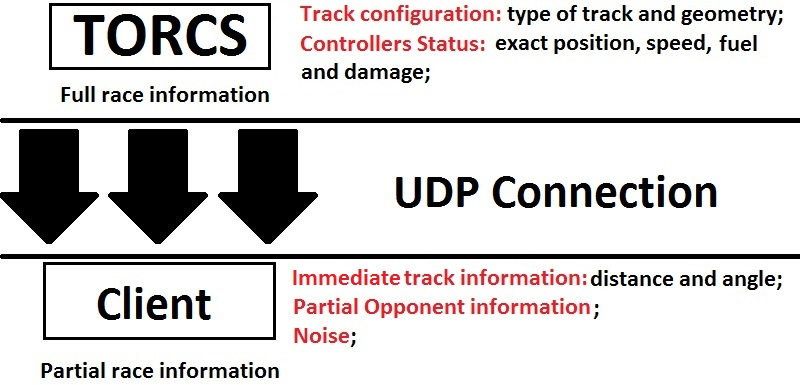
\includegraphics[width=250pt]{Figure1.jpg}
%	\caption{Available data inside TORCS becoming data accessible to the client}
%	\label{Fig:Comm}

% \end{figure}

% Race tracks are categorized into \emph{Road}, \emph{Dirt} and \emph{Oval} inside TORCS. The races from the SCRC take place in track types decided by the organization of the championship, information which is not provided to the participants and that may incorporate maps that are unknown to them. The competition adopts a structure that gathers a \textit{Warm-up} stage, a \textit{Qualifier} stage and a \textit{Final} race. Noise can be introduced in the sensors, option that is present during the actual competition. The complete sensorial input information and all the details concerning the race stages and types are presented at the Simulated Car Racing Championship Competition Software Manual~\cite{SCRC}.

% The reason why TORCS presents itself as a satisfactory AI benchmark, in combination with SCR, is because even	though there are multiple possibilities on how the sensorial input received from the server can be translated into the behavior of the actuators, they can all be compared in a race, which has a robust and steady scoring and evaluational system. In other words, there are many different approaches concerning how to teach the racer encoded by the developers to drive in a racing competition only with the information given by the sensors, and the metric to that issue is the performance on the race itself.



% \section{\textbf{Related Works and State of the Art}} \label{sec:Related}

SCR controllers have been developed using AI techniques, such as neural networks, fuzzy logic, potential fields, and genetic algorithms~\cite{Loiacono:2012:LEA:2212908.2212953}. In the competition, the race track is initially unknown and it several drivers incorporate machine learning procedures to improve their performance~\cite{2009} advantage, which can essentially be \emph{online} or \emph{offline}. Online systems learn by moving about the environment and observing the results while offline ones learn solely by simulating actions within an internal model~\cite{mitchell_1997}.

\emph{Mr. Racer}, which has won the last three championships (2011 to 2013), employs several heuristics and black-box optimization methods in a a modular structure in order to reproduce human-like mechanisms~\cite{MrRacer}, it applies a Covariance Matrix Adaptation Evolution Strategy (CMA-ES), to evolve parameters offline.

In the GECCO leg of the 2013 competition\footnote{\url{http://www.slideshare.net/dloiacono/gecco13scr}}, \emph{AUTOPIA}'s performance stands out. It implements a fuzzy architecture with gear, steering and speed control modules which are optimized offline by a genetic algorithm and an online learning mechanism for landmarking lane exit points to avoid leaving the track~\cite{AUTOPIA}.

Not surprisingly, other participants also use combinations of offline and online learning and modular approaches~\cite{2009,DIEGO,Exp}. Modularity has the clear advantage of independent development and optimization\cite{MrRacer,AUTOPIA2009}, and one of the simplest models for implementing different behaviors is a finite-state machine.

\subsection{Finite-State Machines}%
A FSM is a mathematical model with a finite number of states that can transition from one to another, and a FSM whose output values are determined solely by its current state is a Moore machine~\cite{Ajzerman}. FSMs have been widely used in AI application~\cite{Millington:2006:FSM}, mostly due to its inherent characteristics of flexibility, modularity, and intuitive behavior, among others~\cite{Buckland:2005:AI}.

States are usually implemented with hard-coded rules concerning a specific situation~\cite{Buckland:2005:AI}, which in turn demands small amounts of processor time, and can be easily implemented in different manners. The different driving behaviors can then be coded in parallel with less effort, and easily translated into different states of a FSM. Such approach has successfully been used in SCR~\cite{2009,DIEGO}.

The proper configuration of states and transitions, however, are a more complex problem. Several possible solutions exist, and machine learning techniques can readily be applied.

\subsection{Genetic Algorithms}

GAs are a particular kind of genetic optimization mechanism, inspired by evolutionary algorithms inspired by Darwin's theory of natural selection~\cite{GA}. They are probabilistic search procedures designed to work on large spaces~\cite{goldberg1988}, and have been successful applications in many areas~\cite{GABIO,GAECO,stanley_real-time_2005,pedrycz_genetic_2005}.

GAs work by generating successor solutions by repeatedly mutating and recombining parts of the best currently known solutions, replacing a fraction of the population by offspring~\cite{mitchell_1997}. This is interesting because it works with little information on the problem's domain, the only requirements related specifically to the problem are a representation of a solution for a problem and a function for evaluating it's quality (fitness).

In the context of a self-driving car controller, a solution can be seen as a representation of the driver's parameters and the fitness a measure of its performance, considering speed, safety, fuel consumption, or whatever is the developer's interest. Considering SCR, the usual fitness is the distance driven during the given simulation time~\cite{2009}.
